% This file was created by matplotlib2tikz v0.6.18.
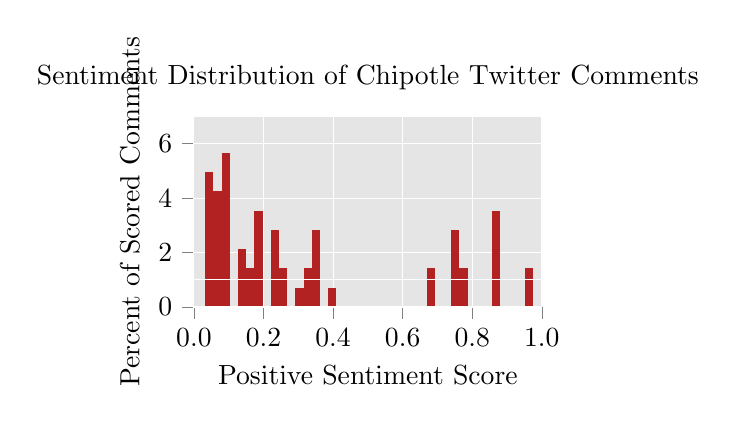
\begin{tikzpicture}

\definecolor{color0}{rgb}{0.698039215686274,0.133333333333333,0.133333333333333}

\begin{axis}[
axis background/.style={fill=white!89.80392156862746!black},
axis line style={white},
height=4cm,
tick align=outside,
tick pos=left,
title={Sentiment Distribution of Chipotle Twitter Comments},
width=6cm,
x grid style={white},
xlabel={Positive Sentiment Score},
xmajorgrids,
xmin=0, xmax=1,
xtick={0,0.2,0.4,0.6,0.8,1},
xticklabels={0.0,0.2,0.4,0.6,0.8,1.0},
y grid style={white},
ylabel={Percent of Scored Comments},
ymajorgrids,
ymin=0, ymax=7
]
\draw[fill=color0,draw opacity=0] (axis cs:0.0325786024332047,0) rectangle (axis cs:0.0561354793608189,4.95255237038259);
\draw[fill=color0,draw opacity=0] (axis cs:0.0561354830861092,0) rectangle (axis cs:0.0796923637390137,4.24504488889936);
\draw[fill=color0,draw opacity=0] (axis cs:0.0796923488378525,0) rectangle (axis cs:0.103249229490757,5.6600589567827);
\draw[fill=color0,draw opacity=0] (axis cs:0.103249236941338,0) rectangle (axis cs:0.126806110143661,0);
\draw[fill=color0,draw opacity=0] (axis cs:0.126806110143661,0) rectangle (axis cs:0.150362983345985,2.12252278010595);
\draw[fill=color0,draw opacity=0] (axis cs:0.150362983345985,0) rectangle (axis cs:0.173919871449471,1.41501429165433);
\draw[fill=color0,draw opacity=0] (axis cs:0.173919856548309,0) rectangle (axis cs:0.197476729750633,3.53753796684326);
\draw[fill=color0,draw opacity=0] (axis cs:0.197476744651794,0) rectangle (axis cs:0.221033617854118,0);
\draw[fill=color0,draw opacity=0] (axis cs:0.221033602952957,0) rectangle (axis cs:0.244590476155281,2.83003037347461);
\draw[fill=color0,draw opacity=0] (axis cs:0.244590491056442,0) rectangle (axis cs:0.268147379159927,1.41501429165433);
\draw[fill=color0,draw opacity=0] (axis cs:0.268147379159927,0) rectangle (axis cs:0.291704267263412,0);
\draw[fill=color0,draw opacity=0] (axis cs:0.291704297065735,0) rectangle (axis cs:0.315261155366898,0.707508040910703);
\draw[fill=color0,draw opacity=0] (axis cs:0.315261125564575,0) rectangle (axis cs:0.33881801366806,1.41501429165433);
\draw[fill=color0,draw opacity=0] (axis cs:0.33881801366806,0) rectangle (axis cs:0.362374871969223,2.83003216364281);
\draw[fill=color0,draw opacity=0] (axis cs:0.362374871969223,0) rectangle (axis cs:0.385931760072708,0);
\draw[fill=color0,draw opacity=0] (axis cs:0.385931760072708,0) rectangle (axis cs:0.409488648176193,0.707507145827166);
\draw[fill=color0,draw opacity=0] (axis cs:0.409488677978516,0) rectangle (axis cs:0.433045536279678,0);
\draw[fill=color0,draw opacity=0] (axis cs:0.433045506477356,0) rectangle (axis cs:0.456602394580841,0);
\draw[fill=color0,draw opacity=0] (axis cs:0.456602394580841,0) rectangle (axis cs:0.480159282684326,0);
\draw[fill=color0,draw opacity=0] (axis cs:0.480159282684326,0) rectangle (axis cs:0.503716170787811,0);
\draw[fill=color0,draw opacity=0] (axis cs:0.503716170787811,0) rectangle (axis cs:0.527272999286652,0);
\draw[fill=color0,draw opacity=0] (axis cs:0.527272939682007,0) rectangle (axis cs:0.550829827785492,0);
\draw[fill=color0,draw opacity=0] (axis cs:0.550829887390137,0) rectangle (axis cs:0.574386775493622,0);
\draw[fill=color0,draw opacity=0] (axis cs:0.574386715888977,0) rectangle (axis cs:0.597943603992462,0);
\draw[fill=color0,draw opacity=0] (axis cs:0.597943663597107,0) rectangle (axis cs:0.621500551700592,0);
\draw[fill=color0,draw opacity=0] (axis cs:0.621500492095947,0) rectangle (axis cs:0.645057380199432,0);
\draw[fill=color0,draw opacity=0] (axis cs:0.645057439804077,0) rectangle (axis cs:0.668614268302917,0);
\draw[fill=color0,draw opacity=0] (axis cs:0.668614268302917,0) rectangle (axis cs:0.692171156406403,1.41501429165433);
\draw[fill=color0,draw opacity=0] (axis cs:0.692171096801758,0) rectangle (axis cs:0.715727984905243,0);
\draw[fill=color0,draw opacity=0] (axis cs:0.715728044509888,0) rectangle (axis cs:0.739284932613373,0);
\draw[fill=color0,draw opacity=0] (axis cs:0.739284873008728,0) rectangle (axis cs:0.762841761112213,2.83002858330866);
\draw[fill=color0,draw opacity=0] (axis cs:0.762841820716858,0) rectangle (axis cs:0.786398649215698,1.41501787199301);
\draw[fill=color0,draw opacity=0] (axis cs:0.786398649215698,0) rectangle (axis cs:0.809955537319183,0);
\draw[fill=color0,draw opacity=0] (axis cs:0.809955477714539,0) rectangle (axis cs:0.833512365818024,0);
\draw[fill=color0,draw opacity=0] (axis cs:0.833512425422668,0) rectangle (axis cs:0.857069313526154,0);
\draw[fill=color0,draw opacity=0] (axis cs:0.857069253921509,0) rectangle (axis cs:0.880626142024994,3.53753572913583);
\draw[fill=color0,draw opacity=0] (axis cs:0.880626201629639,0) rectangle (axis cs:0.904183089733124,0);
\draw[fill=color0,draw opacity=0] (axis cs:0.904183089733124,0) rectangle (axis cs:0.927739918231964,0);
\draw[fill=color0,draw opacity=0] (axis cs:0.927739858627319,0) rectangle (axis cs:0.951296746730804,0);
\draw[fill=color0,draw opacity=0] (axis cs:0.951296806335449,0) rectangle (axis cs:0.974853694438934,1.41501429165433);
\path [draw=white, fill opacity=0] (axis cs:0,0)
--(axis cs:0,7);

\path [draw=white, fill opacity=0] (axis cs:1,0)
--(axis cs:1,7);

\path [draw=white, fill opacity=0] (axis cs:0,0)
--(axis cs:1,0);

\path [draw=white, fill opacity=0] (axis cs:0,1)
--(axis cs:1,1);

\end{axis}

\end{tikzpicture}